\documentclass[aspectratio=169]{beamer}\usepackage[]{graphicx}\usepackage[]{xcolor}
% maxwidth is the original width if it is less than linewidth
% otherwise use linewidth (to make sure the graphics do not exceed the margin)
\makeatletter
\def\maxwidth{ %
  \ifdim\Gin@nat@width>\linewidth
    \linewidth
  \else
    \Gin@nat@width
  \fi
}
\makeatother
\usepackage{xcolor}
\definecolor{lightblue}{RGB}{173, 216, 230}
\definecolor{lightyellow}{RGB}{255, 255, 224}
\definecolor{lightgreen}{RGB}{144, 238, 144}
\definecolor{lightyellow}{RGB}{255, 255, 153}
\definecolor{lightgray}{RGB}{211, 211, 211}
\definecolor{fgcolor}{rgb}{0.345, 0.345, 0.345}
\newcommand{\hlnum}[1]{\textcolor[rgb]{0.686,0.059,0.569}{#1}}%
\newcommand{\hlsng}[1]{\textcolor[rgb]{0.192,0.494,0.8}{#1}}%
\newcommand{\hlcom}[1]{\textcolor[rgb]{0.678,0.584,0.686}{\textit{#1}}}%
\newcommand{\hlopt}[1]{\textcolor[rgb]{0,0,0}{#1}}%
\newcommand{\hldef}[1]{\textcolor[rgb]{0.345,0.345,0.345}{#1}}%
\newcommand{\hlkwa}[1]{\textcolor[rgb]{0.161,0.373,0.58}{\textbf{#1}}}%
\newcommand{\hlkwb}[1]{\textcolor[rgb]{0.69,0.353,0.396}{#1}}%
\newcommand{\hlkwc}[1]{\textcolor[rgb]{0.333,0.667,0.333}{#1}}%
\newcommand{\hlkwd}[1]{\textcolor[rgb]{0.737,0.353,0.396}{\textbf{#1}}}%
\let\hlipl\hlkwb

\usepackage{framed}
\makeatletter
\newenvironment{kframe}{%
 \def\at@end@of@kframe{}%
 \ifinner\ifhmode%
  \def\at@end@of@kframe{\end{minipage}}%
  \begin{minipage}{\columnwidth}%
 \fi\fi%
 \def\FrameCommand##1{\hskip\@totalleftmargin \hskip-\fboxsep
 \colorbox{shadecolor}{##1}\hskip-\fboxsep
     % There is no \\@totalrightmargin, so:
     \hskip-\linewidth \hskip-\@totalleftmargin \hskip\columnwidth}%
 \MakeFramed {\advance\hsize-\width
   \@totalleftmargin\z@ \linewidth\hsize
   \@setminipage}}%
 {\par\unskip\endMakeFramed%
 \at@end@of@kframe}
\makeatother

\definecolor{shadecolor}{rgb}{.97, .97, .97}
\definecolor{messagecolor}{rgb}{0, 0, 0}
\definecolor{warningcolor}{rgb}{1, 0, 1}
\definecolor{errorcolor}{rgb}{1, 0, 0}
\newenvironment{knitrout}{}{} % an empty environment to be redefined in TeX

\usepackage{alltt}




\input{slides-setup-whiteBG.tex}

\title{Clustering \& Classification using ANNs}
\author{\texorpdfstring{Adriana-Stefania Ciupeanu\newline University of Manitoba\newline}{Adriana-Stefania Ciupeanu}}
\date{}
\IfFileExists{upquote.sty}{\usepackage{upquote}}{}
\begin{document}

%%%%%%%%%%%%%%%%%%%%%%%%%%%%%%%%%
%%%%%%%%%%%%%%%%%%%%%%%%%%%%%%%%%
%% TITLE AND OUTLINE
%%%%%%%%%%%%%%%%%%%%%%%%%%%%%%%%%
%%%%%%%%%%%%%%%%%%%%%%%%%%%%%%%%%
\titlepagewithfigure{FIGS-slides-admin/Gemini_Generated_Image_pbzl1mpbzl1mpbzl.jpeg}

%%%%%%%%%%%%%%%%%%%%%%%%%%%%%%%%
%% Biological background
%%%%%%%%%%%%%%%%%%%%%%%%%%%%%%%%
\outlinepage{FIGS-slides-admin/Gemini_Generated_Image_yegaxcyegaxcyega.jpeg}

%%%%%%%%%%%%%%%%%%%
%%%%%%%%%%%%%%%%%%%
%%%%%%%%%%%%%%%%%%%
%%%%%%%%%%%%%%%%%%%
%%%%%%%%%%%%%%%%%%%
%%%%%%%%%%%%%%%%%%%
%%%%%%%%%%%%%%%%%%%
%%%%%%%%%%%%%%%%%%%
\section{Motivation}

\newSectionSlide{FIGS-slides-admin/Gemini_Generated_Image_yegaxcyegaxcyega.jpeg}
\begin{frame}{Why Neural Networks?}

\begin{columns}
\column{0.5\textwidth}
\textbf{Applications:}
\begin{itemize}
    \item Image recognition
    \item Natural language processing
    \item Time series prediction
    \item Complex classification
\end{itemize}

\column{0.5\textwidth}
\textbf{Key Advantages:}
\begin{itemize}
    \item Learn non-linear patterns
    \item Automatic feature learning
    \item Surprisingly flexible
    \item Proven in practice
\end{itemize}
\end{columns}
\end{frame}

%%%%%%%%%%%%%%%%%%%
%%%%%%%%%%%%%%%%%%%
%%%%%%%%%%%%%%%%%%%
%%%%%%%%%%%%%%%%%%%
%%%%%%%%%%%%%%%%%%%
%%%%%%%%%%%%%%%%%%%
%%%%%%%%%%%%%%%%%%%
%%%%%%%%%%%%%%%%%%%

\section{Biological Background}
\newSectionSlide{FIGS-slides-admin/Gemini_Generated_Image_yegaxcyegaxcyega.jpeg}

\begin{frame}{The Biological Neuron}
Many machine learning methods inspired by biology, e.g., the (human) brain \\
\vfill 
Our brain has $~ 10^{11}$ neurons, each of which communicates (is connected) to $~$ $10^4$ other neurons
\vfill

\begin{minipage}{.6\textwidth}
\begin{figure}
\includegraphics[scale=0.2]{FIGS/neuron_fig.png}
\end{figure}
\end{minipage}%
\begin{minipage}{.4\textwidth}
\begin{itemize}
    \item \textbf{Dendrites}: receive signals
    \item \textbf{Cell body}: integrates signals
    \item \textbf{Axon}: transmits output
    \item \textbf{Synapses}: modifiable connections
\end{itemize}
\end{minipage}

\end{frame}


\begin{frame}{Learning in Brains and Neural Networks: Synaptic Plasticity}
\textbf{Synaptic Plasticity}: The ability of connections between neurons to change strength based on activity.
\vfill
\begin{center}
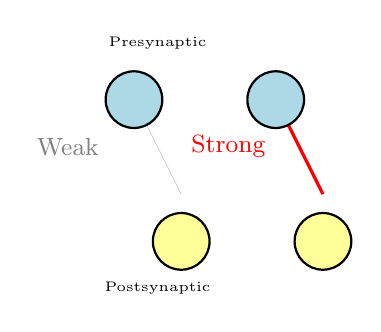
\begin{tikzpicture}[scale=1.2]
    % Weak connection
    \draw[very thin, gray, opacity=0.5] (0, 2) -- (0.5, 1);
    \node[gray, font=\small] at (-0.7, 1.5) {Weak};
    
    % Strong connection  
    \draw[very thick, red] (1.5, 2) -- (2, 1);
    \node[red, font=\small] at (1, 1.5) {Strong};
    
    % Neurons
    \draw[fill=lightblue, thick] (0, 2) circle (0.3cm);
    \draw[fill=lightblue, thick] (1.5, 2) circle (0.3cm);
    
    \draw[fill=lightyellow, thick] (0.5, 0.5) circle (0.3cm);
    \draw[fill=lightyellow, thick] (2, 0.5) circle (0.3cm);
    
    % Labels
    \node[font=\tiny] at (0.25, 2.6) {Presynaptic};
    \node[font=\tiny] at (0.25, 0) {Postsynaptic};
\end{tikzpicture}
\end{center}
\vfill

\textbf{Hebbian Principle}: ``Neurons that fire together, wire together''

\vfill

\textbf{Why this matters for artificial neural networks:}
\begin{itemize}
    \item Connection strength $\leftrightarrow$ \textbf{weights} in our network
    \item Learning means \textbf{adjusting weights} based on activity patterns
    \item Backpropagation is the artificial version of synaptic plasticity
\end{itemize}
\end{frame}



%%%%%%%%%%%%%%%%%%%
%%%%%%%%%%%%%%%%%%%
%%%%%%%%%%%%%%%%%%%
%%%%%%%%%%%%%%%%%%%
%%%%%%%%%%%%%%%%%%%
%%%%%%%%%%%%%%%%%%%
%%%%%%%%%%%%%%%%%%%
%%%%%%%%%%%%%%%%%%%
\section{Neural networks (the perceptron)}
\newSectionSlide{FIGS-slides-admin/Gemini_Generated_Image_5g0m5e5g0m5e5g0m.jpeg}

\begin{frame}{Artificial neural network (ANN) - from \href{https://en.wikipedia.org/wiki/Artificial_neural_network}{Wikipedia}}
    \begin{quote}
    \textbf{Artificial neural networks} (ANNs) are computing systems inspired by the biological neural networks that constitute animal brains
    \vfill
    An ANN is based on a collection of connected units or nodes called \textbf{artificial neurons}, which loosely model the neurons in a biological brain. Each connection, like the synapses in a biological brain, can transmit a signal to other neurons. An artificial neuron receives signals then processes them and can signal neurons connected to it. The ``signal" at a connection is a real number, and the output of each neuron is computed by some non-linear function of the sum of its inputs. The connections are called edges. Neurons and edges typically have a weight that adjusts as learning proceeds. The weight increases or decreases the strength of the signal at a connection. Neurons may have a threshold such that a signal is sent only if the aggregate signal crosses that threshold.
    \end{quote}
\end{frame}


\begin{frame}{The perceptron}
    One of the first neural networks (invented 1943, implemented 1957), made for simple classification tasks, for example recognising letters or numbers
    \vfill
    Two layers: the \emph{input} layer (the \emph{retina}) and the \emph{output} layer
    \vfill
    Inputs are 0 or 1, so are outputs
\end{frame}

\begin{frame}{From Biology to Computation}

\begin{minipage}{0.6\textwidth}

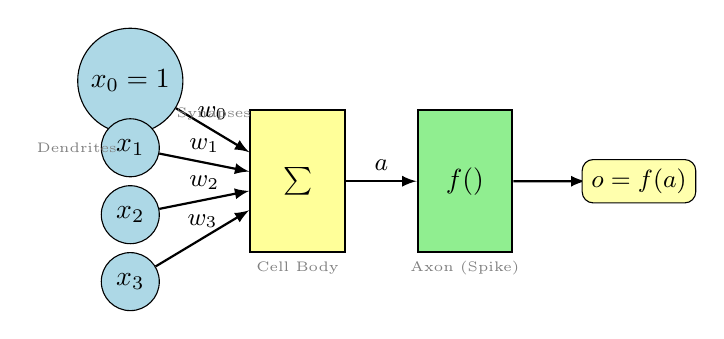
\begin{tikzpicture}[scale=0.85]
    % Inputs with biological labels
    \node[circle, draw, fill=lightblue] (x0) at (0, 2) {$x_0=1$};
    \node[circle, draw, fill=lightblue] (x1) at (0, 1) {$x_1$};
    \node[circle, draw, fill=lightblue] (x2) at (0, 0) {$x_2$};
    \node[circle, draw, fill=lightblue] (x3) at (0, -1) {$x_3$};
    
    \node[font=\tiny, gray] at (-0.8, 1) {Dendrites};
    
    % Summation - representing cell body integration
    \node[draw, thick, minimum width=1.2cm, minimum height=1.8cm, fill=lightyellow] (sum) at (2.5, 0.5) {$\sum$};
    \node[font=\tiny, gray] at (2.5, -0.8) {Cell Body};
    
    % Weights with visual emphasis
    \draw[-latex, thick] (x0) -- (sum) node[midway, above, font=\small] {$w_0$};
    \draw[-latex, thick] (x1) -- (sum) node[midway, above, font=\small] {$w_1$};
    \draw[-latex, thick] (x2) -- (sum) node[midway, above, font=\small] {$w_2$};
    \draw[-latex, thick] (x3) -- (sum) node[midway, above, font=\small] {$w_3$};
    
    \node[font=\tiny, gray] at (1.25, 1.5) {Synapses};
    
    % Activation function - representing axon
    \node[draw, thick, minimum width=1.2cm, minimum height=1.8cm, fill=lightgreen] (act) at (5, 0.5) {$f()$};
    \node[font=\tiny, gray] at (5, -0.8) {Axon (Spike)};
    \draw[-latex, thick] (sum) -- (act) node[midway, above, font=\small] {$a$};
    
    % Output
    \draw[-latex, thick] (act) -- (6.8, 0.5);
    \node[font=\small, fill=lightyellow!80, draw, rounded corners] at (7.6, 0.5) {$o = f(a)$};
\end{tikzpicture}
\end{minipage}%
\begin{minipage}{.4\textwidth}
\begin{align*}
a &= \sum_{i=0}^{n} w_i x_i \quad \text{(weighted sum)} \\
o &= f(a) \quad \text{(activation)}
\end{align*}
\end{minipage}



\begin{tabular}{lll}
\toprule
\textbf{Biological Neuron} & $\leftrightarrow$ & \textbf{Artificial Neuron} \\
\midrule
Dendrites receive signals & $\leftrightarrow$ & Inputs $x_i$ \\
Synaptic strength & $\leftrightarrow$ & Weights $w_i$ \\
Cell body integrates & $\leftrightarrow$ & Summation $\sum w_i x_i$ \\
Action potential threshold & $\leftrightarrow$ & Activation $f(a)$ \\
Axon fires/doesn't fire & $\leftrightarrow$ & Output $o$ \\
\bottomrule
\end{tabular}
\end{frame}

\begin{frame}{}
    \begin{center}
        \def\hhskip{8cm}
        \def\vvskip{2.75cm}
        \begin{tikzpicture}[scale=0.75, 
		every node/.style={transform shape},
		auto,
		cloud/.style={minimum width={width("N-1")+2pt},
			draw, ellipse},
		connected/.style={dotted,-}]
		%% Input nodes
		\node [cloud] at (0,0*\vvskip) (i1) {$0\lor 1$};
		\node [cloud] at (0,-1*\vvskip) (i2) {$0\lor 1$};
		\node [cloud] at (0,-2*\vvskip) (i3) {$0\lor 1$};
		\node [cloud] at (0,-3*\vvskip) (i4) {$0\lor 1$};
		%% Output nodes
		\node [cloud] at (1*\hhskip,-0.5*\vvskip) (o1) {$\sum$};
		\node [cloud] at (1*\hhskip,-1.5*\vvskip) (o2) {$\sum$};
		\node [cloud] at (1*\hhskip,-2.5*\vvskip) (o3) {$\sum$};
		%% Arcs
		\path [line] (i1) to node [midway, above] (TextNode) {} (o1);
		\path [line] (i1) to node [midway, above] (TextNode) {} (o2);
		\path [line] (i1) to node [midway, above] (TextNode) {} (o3);
		\path [line] (i2) to node [midway, above] (TextNode) {} (o1);
		\path [line] (i2) to node [midway, above] (TextNode) {} (o2);
		\path [line] (i2) to node [midway, above] (TextNode) {} (o3);
		\path [line] (i3) to node [midway, above] (TextNode) {} (o1);
		\path [line] (i3) to node [midway, above] (TextNode) {} (o2);
		\path [line] (i3) to node [midway, above] (TextNode) {} (o3);
		\path [line] (i4) to node [midway, above] (TextNode) {} (o1);
		\path [line] (i4) to node [midway, above] (TextNode) {} (o2);
		\path [line] (i4) to node [midway, above] (TextNode) {} (o3);
        %% Arrows out of output nodes
		\path [line] (o1) to node [midway, above] (TextNode) {$0\lor 1$} (1.2*\hhskip,-0.5*\vvskip);
		\path [line] (o2) to node [midway, above] (TextNode) {$0\lor 1$} (1.2*\hhskip,-1.5*\vvskip);
		\path [line] (o3) to node [midway, above] (TextNode) {$0\lor 1$} (1.2*\hhskip,-2.5*\vvskip);
        %% Some labels
        \node[align=left] at (0.5*\hhskip,0) {Connections};
        \node[align=left] at (0*\hhskip,0.33*\vvskip) {Retina};
        \node[align=left] at (1*\hhskip,0.33*\vvskip) {Output layer};
	\end{tikzpicture}
    \end{center}
    The connections into the output layer are called \emph{synapses}, they are modifiable
\end{frame}


\begin{frame}{The activation function}
    \begin{center}
        \def\hhskip{8cm}
        \def\vvskip{2cm}
        \begin{tikzpicture}[scale=0.75, 
		every node/.style={transform shape},
		auto,
		cloud/.style={minimum width={width("N-1")+2pt},
			draw, ellipse},
		connected/.style={dotted,-}]
		%% Input nodes
		\node [cloud] at (0,0*\vvskip) (i1) {$x_0$};
		\node [cloud] at (0,-1*\vvskip) (i2) {$x_1$};
		\node [cloud] at (0,-2*\vvskip) (i3) {$x_i$};
		\node [cloud] at (0,-3*\vvskip) (i4) {$x_\ell$};
		%% Output nodes
		\node [cloud] at (1*\hhskip,-1.5*\vvskip) (o1) {$a_j=\sum_{i=1}^I w_{ij}x_i$};
		%% Arcs
		\path [line] (i1) to node [midway, above] (TextNode) {$w_{1j}$} (o1);
		\path [line] (i2) to node [midway, above] (TextNode) {$w_{2j}$} (o1);
		\path [line] (i3) to node [midway, above] (TextNode) {$w_{ij}$} (o1);
		\path [line] (i4) to node [midway, above] (TextNode) {$w_{I j}$} (o1);
        %% Arrows out of output nodes
		\path [line] (o1) to node [midway, above] (TextNode) {$o_j=f(a_j)$} (1.5*\hhskip,-1.5*\vvskip);
	\end{tikzpicture}
    \end{center}
    Here,
    \[
        f(a_j)= \begin{cases}
            0 & \text{if }a_j\leq 0 \\
            1 & \text{if }a_j>0
        \end{cases}
    \]
\end{frame}

\begin{frame}{The activation function}
    We have $I$ input neurons taking values $0$ or $1$, $O$ output neurons taking values $0$ or $1$, weights $W=[w_{ij}]\in\M_{IO}$ and a threshold function $f$
    \vfill
    More generally, use a threshold $\theta_j$ for each output neuron
    \[
        o_j= \begin{cases}
            0 & \text{if }a_j\leq \theta_j \\
            1 & \text{if }a_j>\theta_j
        \end{cases}
    \]
    \vfill
    The thresholds (or \emph{response bias}) and the weights are modifiable by learning. To do that easily for the threshold, consider an input neuron that is always on, say neuron 0, and set weights $w_{0j}=-\theta_j$, making the weights matrix an $(I+1)\times O$-matrix
\end{frame}


\begin{frame}
    Another way to write the activation is 
    \[
        o_j= \begin{cases}
            0 & \text{if }a_j+w_{0j}\leq 0 \\
            1 & \text{if }a_j+w_{0j}>0
        \end{cases}
    \]
    where $w_{0j}=-\theta_j$
\end{frame}

\begin{frame}{Common Activation Functions}

\begin{center}
\small
\begin{tabular}{llc}
\toprule
\textbf{Function} & \textbf{Definition} & \textbf{Range} \\
\midrule
Sigmoid & $\sigma(a) = \frac{1}{1+e^{-a}}$ & $(0, 1)$ \\
Tanh & $\tanh(a) = \frac{e^a - e^{-a}}{e^a + e^{-a}}$ & $(-1, 1)$ \\
ReLU & $f(a) = \max(0, a)$ & $[0, \infty)$ \\
Linear & $f(a) = a$ & $(-\infty, \infty)$ \\
\bottomrule
\end{tabular}
\end{center}

\vfill

\textbf{Key insight}:
\begin{itemize}
    \item Hidden layers: Use ReLU, tanh, or sigmoid
    \item Output layer: Match to task (linear, sigmoid, softmax)
\end{itemize}

\end{frame}


\begin{frame}{Why Non-Linearity Matters}

\textbf{Without activation:}
\[
o = W_2(W_1 x) = (W_2 W_1) x = W_{\text{combined}} x \quad \text{(linear!)}
\]

\vfill
\textbf{Result}: Can only learn linear patterns

\vfill
\textbf{Solution}: Apply non-linear function $f()$ after each sum

\end{frame}

\begin{frame}{Single Neuron vs. Network}

\textbf{Limitation}: Single neuron = linear decision boundary

\vfill

\begin{center}
\textbf{Single Neuron}

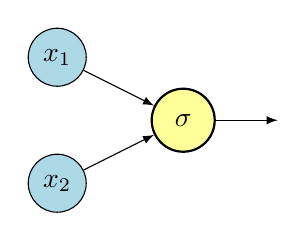
\begin{tikzpicture}[scale=0.8]
    \node[circle, draw, fill=lightblue] (x1) at (0, 1) {$x_1$};
    \node[circle, draw, fill=lightblue] (x2) at (0, -1) {$x_2$};
    \node[draw, circle, thick, minimum width=0.8cm, fill=lightyellow] (n) at (2, 0) {$\sigma$};
    \draw[-latex] (x1) -- (n);
    \draw[-latex] (x2) -- (n);
    \draw[-latex] (n) -- (3.5, 0);
\end{tikzpicture}

\vfill
\textbf{Multi-Layer Network}

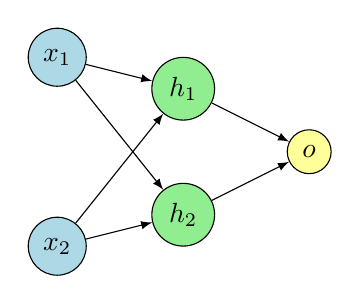
\begin{tikzpicture}[scale=0.8]
    % Input
    \node[circle, draw, fill=lightblue] (x1) at (0, 1.5) {$x_1$};
    \node[circle, draw, fill=lightblue] (x2) at (0, -1.5) {$x_2$};
    
    % Hidden
    \node[circle, draw, fill=lightgreen] (h1) at (2, 1) {$h_1$};
    \node[circle, draw, fill=lightgreen] (h2) at (2, -1) {$h_2$};
    
    % Output
    \node[circle, draw, fill=lightyellow] (o) at (4, 0) {$o$};
    
    % Connections
    \draw[-latex] (x1) -- (h1);
    \draw[-latex] (x1) -- (h2);
    \draw[-latex] (x2) -- (h1);
    \draw[-latex] (x2) -- (h2);
    \draw[-latex] (h1) -- (o);
    \draw[-latex] (h2) -- (o);
\end{tikzpicture}
\end{center}
\end{frame}

\begin{frame}{The Learning Problem}

\textbf{Goal}: Adjust weights to minimize prediction error

\begin{center}
\textbf{Forward Pass} (predict)
\[\text{input} \xrightarrow{\text{weights}} \text{hidden} \xrightarrow{\text{weights}} \text{output}\]

\vspace{0.5cm}

\textbf{Backward Pass} (learn)
\[\text{Error} \xrightarrow{\text{gradients}} \text{update weights}\]
\end{center}

\vfill

\textbf{Loss function}: 
\[
\text{Loss} = \frac{1}{N} \sum_{i=1}^{N} (y_i - \hat{y}_i)^2
\]
\end{frame}


\begin{frame}{Learning something simple}
    The aim is to adjust the synaptic weights so that the proper response is provided to a given stimulus
    \vfill
    Let us first do a simple example: the OR truth table
    \begin{center}
        \begin{tabular}{cccc}
            0 & 0 & $\mapsto$ & 0 \\
            1 & 0 & $\mapsto$ & 1 \\
            0 & 1 & $\mapsto$ & 1 \\
            1 & 1 & $\mapsto$ & 1 \\
        \end{tabular}
    \end{center}
    So we have two neurons in the retina and a single output neuron
\end{frame}

\begin{frame}{Supervised learning}
    (From R. Rojas)
    \begin{quote}
    \textbf{Supervised learning}: method in which some input vectors are collected and presented to the network. The output computed by the network is observed and the deviation from the expected answer is measured
    \vskip0.5cm
    The weights are corrected according to the magnitude of the error in the way defined by the learning algorithm
    \vskip0.5cm
    Also called \emph{learning with a teacher}, since a control process knows the correct answer for the set of selected input vectors
    \end{quote}
\end{frame}

\begin{frame}{Further distinctions in supervised learning methods}
    Methods with \emph{reinforcement} or \emph{error correction} 
    \vfill
    \begin{itemize}
        \item \textbf{Reinforcement learning}: used when after each presentation of an input-output example, we only know whether the network produces the desired result or not. 
        Weights are updated based on this information (i.e., the Boolean values true or false), so only the input vector can be used for weight correction
        \vfill
        \item In learning with \textbf{error correction}, the
        magnitude of the error, together with the input vector, determines the magnitude of the corrections to the weights. In many cases, we try to eliminate the error in a single correction step
    \end{itemize}
\end{frame}

\begin{frame}{A first learning algorithm}
    Suppose the training set consists of two sets of points $P$ and $N$
    \vfill
    \begin{itemize}
        \item \textbf{start:} Generate random weight vector $w_0$; set $t := 0$
        \vfill
        \item \textbf{test:} A vector $x\in P\cup N$ is selected randomly
        \begin{itemize}
            \item if $x\in P$ and $\langle w_t,x\rangle > 0$ go to \textbf{test}
            \item if $x\in P$ and $\langle w_t,x\rangle\leq 0$ go to \textbf{add}
            \item if $x\in N$ and $\langle w_t,x\rangle < 0$ go to \textbf{test}
            \item if $x\in N$ and $\langle w_t,x\rangle \geq 0$ go to \textbf{subtract}
        \end{itemize}
        \vfill
        \item \textbf{add:} set $w_{t+1} = w_t + x$ and $t := t + 1$, goto \textbf{test}
        \vfill
        \item \textbf{subtract:} set $w_{t+1} = w_t - x$ and $t := t + 1$, goto \textbf{test}
    \end{itemize}
\end{frame}



\begin{frame}{Widrow-Hoff learning rule}
    Need to provide the correct answer, i.e., this is a supervised learning rule
    \vfill
    An output cell only learns if it is mistaken
    \vfill
    Present random inputs and apply the rule if the output does not match the known output
\end{frame}

\begin{frame}{Widrow-Hoff learning rule}
    \begin{equation}\label{eq:WidrowHoff}
        w_{ij}^{(t+1)} = w_{ij}^{(t)}+\eta(t_j-o_j)x_j = w_{ij}^{(t)}+\Delta w_{ij}        
    \end{equation}
    with
    \begin{itemize}
        \item $\Delta w_{ij}$ correction to add to the weight $w_{ij}$
        \item $x_i$: value ($0$ or $1$) of the $i$th retinal cell
        \item $o_j$: response of the $j$th output cell
        \item $t_j$ target response (correct desired response)
        \item $w_{ij}^{(t)}$: weight of the synapse between the $i$th retinal cell and $j$th output cell at time $t$. Typically initiated at small random values
        \item $\eta$: small positive constant, the \emph{learning constant}
    \end{itemize} 
\end{frame}

\begin{frame}{Understanding Loss Functions}

For a single data point with target $y$ and network output $o$, we measure error as:

\vfill

\textbf{Squared error loss}:
\[
L = \frac{1}{2}(y - o)^2
\]

\vfill

For all $N$ training samples:
\[
L_{\text{total}} = \frac{1}{N} \sum_{i=1}^{N} \frac{1}{2}(y_i - o_i)^2
\]

\vfill

\textbf{Goal of learning}: Minimize this loss by adjusting weights

\vfill

\textbf{How do we minimize?} We compute partial derivatives of the loss with respect to each weight, then move weights in the direction that decreases loss

\end{frame}

\begin{frame}{Derivatives of Common Activation Functions}

We'll need these when using the chain rule. For each activation $f(a)$, we need $\frac{\partial f}{\partial a}$:

\vfill

\begin{center}
\small
\begin{tabular}{lll}
\toprule
\textbf{Function} $f(a)$ & \textbf{Derivative} $f'(a)$ & \textbf{In terms of output } $o = f(a)$ \\
\midrule
Sigmoid & $\sigma(a) = \frac{1}{1+e^{-a}}$ & $\sigma'(a) = \sigma(a)(1-\sigma(a))$ \\
& & $= o(1-o)$ \\
\midrule
Tanh & $\tanh(a)$ & $\tanh'(a) = 1 - \tanh^2(a)$ \\
& & $= 1 - o^2$ \\
\midrule
ReLU & $f(a) = \max(0, a)$ & $f'(a) = \begin{cases} 1 & \text{if } a > 0 \\ 0 & \text{if } a < 0 \end{cases}$ \\
\bottomrule
\end{tabular}
\end{center}

\vfill

\textbf{Key}: We'll use these derivatives in the chain rule for backpropagation
\end{frame}

\begin{frame}{Backpropagation: Single Layer Network}

\textbf{Simple case}: One input layer, one output neuron (no hidden layer)

\vfill

\textbf{Forward pass}:
\begin{align*}
a &= w_1 x_1 + w_2 x_2 + w_0 \quad \text{(weighted sum)} \\
o &= f(a) \quad \text{(apply activation, e.g., sigmoid)}
\end{align*}

\vfill

\textbf{Loss}:
\[
L = \frac{1}{2}(y - o)^2
\]

\vfill

\textbf{Goal}: Find $\frac{\partial L}{\partial w_1}$, $\frac{\partial L}{\partial w_2}$, $\frac{\partial L}{\partial w_0}$ to update weights

\end{frame}

\begin{frame}{Applying the Chain Rule}

To find $\frac{\partial L}{\partial w_1}$, we use the chain rule:

\vfill

\[
\frac{\partial L}{\partial w_1} = \frac{\partial L}{\partial o} \cdot \frac{\partial o}{\partial a} \cdot \frac{\partial a}{\partial w_1}
\]

\vfill

\textbf{Break it into pieces}:

\begin{itemize}
    \item $\displaystyle \frac{\partial L}{\partial o} = \frac{\partial}{\partial o} \left[\frac{1}{2}(y - o)^2\right] = -(y - o)$
    
    \vfill
    
    \item $\displaystyle \frac{\partial o}{\partial a} = f'(a)$ (depends on activation function, e.g., $o(1-o)$ for sigmoid)
    
    \vfill
    
    \item $\displaystyle \frac{\partial a}{\partial w_1} = \frac{\partial}{\partial w_1}(w_1 x_1 + w_2 x_2 + w_0) = x_1$
\end{itemize}

\end{frame}

\begin{frame}{The Gradient}

Putting it together:

\vfill

\[
\frac{\partial L}{\partial w_1} = \underbrace{-(y - o)}_{\text{error}} \cdot \underbrace{f'(a)}_{\text{slope of activation}} \cdot \underbrace{x_1}_{\text{input}}
\]

\vfill

More generally, for any weight $w_i$:

\[
\frac{\partial L}{\partial w_i} = -(y - o) \cdot f'(a) \cdot x_i
\]

\vfill

Similarly, for the bias:

\[
\frac{\partial L}{\partial w_0} = -(y - o) \cdot f'(a) \cdot x_0 = -(y - o) \cdot f'(a)
\]
(since $x_0 = 1$ is the bias input)

\end{frame}

\begin{frame}{Gradient Descent Update}

Once we have the gradient, we update weights using gradient descent:

\vfill

\[
w_i^{(t+1)} = w_i^{(t)} - \eta \frac{\partial L}{\partial w_i}
\]

where $\eta$ is the learning rate (small positive constant, like $\eta = 0.01$)

\vfill

Substituting our gradient:

\[
w_i^{(t+1)} = w_i^{(t)} - \eta \left[-(y - o) \cdot f'(a) \cdot x_i\right]
\]

\[
w_i^{(t+1)} = w_i^{(t)} + \eta (y - o) \cdot f'(a) \cdot x_i
\]

\vfill

\textbf{Compare to Widrow-Hoff}:
\[
w_i^{(t+1)} = w_i^{(t)} + \eta (t - o) x_i
\]

The extra $f'(a)$ term is what makes backprop work with smooth activations!

\end{frame}

\begin{frame}{Comparison: Widrow-Hoff vs Backpropagation}

\begin{center}
\small
\begin{tabular}{lll}
\toprule
\textbf{Aspect} & \textbf{Widrow-Hoff} & \textbf{Backpropagation} \\
\midrule
Layers & Single layer only & \textbf{Any number of layers} \\
\midrule
Update rule & $w \leftarrow w + \eta(t-o)x$ & $w \leftarrow w - \eta \frac{\partial L}{\partial w}$ \\
\midrule
Activation & Step function (0/1) & \textbf{Smooth} (sigmoid, tanh, ReLU) \\
\midrule
Chain rule & Not needed & \textbf{Essential} \\
\midrule
Non-linearity & Ignored & \textbf{Accounted for via } $f'(a)$ \\
\bottomrule
\end{tabular}
\end{center}

\vfill

Backpropagation is Widrow-Hoff generalized:
\begin{itemize}
    \item Works with smooth activation functions (not just 0/1)
    \item Uses chain rule to compute gradients through multiple layers
    \item Error term $(t-o)$ becomes $-(y-o) \cdot f'(a)$ to account for saturation
\end{itemize}

\end{frame}


\begin{frame}{Learning OR}
    \begin{center}
        \begin{tabular}{cccc}
        Input & Input & $\to$ & Target \\
        \midrule
            0 & 0 & $\mapsto$ & 0 \\
            1 & 0 & $\mapsto$ & 1 \\
            0 & 1 & $\mapsto$ & 1 \\
            1 & 1 & $\mapsto$ & 1 \\
        \end{tabular}
    \end{center}
    Three cells in the retina (two inputs and the ``dummy'' cell used for the threshold) and one output cell. So inputs and outputs must be
    \begin{center}
        \begin{tabular}{ccccc}
        Input & Input & Const & $\to$ & Target \\
        \midrule
            1 & 0 & 0 & $\mapsto$ & 0 \\
            1 & 1 & 0 & $\mapsto$ & 1 \\
            1 & 0 & 1 & $\mapsto$ & 1 \\
            1 & 1 & 1 & $\mapsto$ & 1 \\
        \end{tabular}
    \end{center}
    Initialise the $3\times 1$ weight matrix $W$ to zero:
    \[
        W=\begin{pmatrix}
            w_0 = -\theta, w_1, w_2
        \end{pmatrix}^T
        = \begin{pmatrix}
            0, 0, 0
        \end{pmatrix}^T
    \]
\end{frame}


\begin{frame}{Iteration 1: Present $[1, 1, 1] \to 1$}

\textbf{Predict}:
\[
a = w_0 \cdot 1 + w_1 \cdot 1 + w_2 \cdot 1 = 0 + 0 + 0 = 0
\]

Since $a = 0 \leq 0$, output $o = 0$. But target is $t = 1$, so error is $1 - 0 = 1$.

\vfill
\textbf{Update weights}:
\begin{align*}
\Delta w_0 &= 0.1 \times 1 \times 1 = 0.1 \\
\Delta w_1 &= 0.1 \times 1 \times 1 = 0.1 \\
\Delta w_2 &= 0.1 \times 1 \times 1 = 0.1
\end{align*}

\vfill
\textbf{New weights}: $w = [0.1, 0.1, 0.1]^T$
\end{frame}

\begin{frame}{Iteration 2: Present $[1, 0, 0] \to 0$}

\textbf{Predict}:
\[
a = 0.1 \cdot 1 + 0.1 \cdot 0 + 0.1 \cdot 0 = 0.1
\]

Since $a = 0.1 > 0$, output $o = 1$. But target is $t = 0$, so error is $0 - 1 = -1$.

\vfill
\textbf{Update}:
\begin{align*}
\Delta w_0 &= 0.1 \times (-1) \times 1 = -0.1 \\
\Delta w_1 &= 0.1 \times (-1) \times 0 = 0 \\
\Delta w_2 &= 0.1 \times (-1) \times 0 = 0
\end{align*}

\vfill
\textbf{New weights}: $w = [0, 0.1, 0.1]^T$ 
\end{frame}


\begin{frame}{And we are done!}
    With the weights
    \[
        W=\begin{pmatrix}
            0\\ 0.1\\ 0.1
        \end{pmatrix}
    \]
    we are done. Indeed
    \begin{center}
        \begin{tabular}{cccccc}
            Input 0 & Input 1 & Input 2 & a & o & Should be \\
            1 & 0 & 0 & 0 & 0 & 0 \\
            1 & 1 & 0 & 0+0.1+0 & 1 & 1 \\
            1 & 0 & 1 & 0+0+0.1 & 1 & 1 \\
            1 & 1 & 1 & 0+0.1+0.1 & 1 & 1 \\
        \end{tabular}
    \end{center}    
\end{frame}

\begin{frame}[fragile]{Setting Up R}

\begin{lstlisting}
# Install once
install.packages("neuralnet")

# Load for session
library(neuralnet)
\end{lstlisting}

\vfill
The \texttt{neuralnet} package provides:
\begin{itemize}
    \item Flexible network specification
    \item Training via backpropagation
    \item Prediction on new data
    \item Network visualization
\end{itemize}
\end{frame}

\begin{frame}[fragile]\frametitle{Using \code{neuralnet} to learn OR}
First, create the truth table
\begin{knitrout}
\definecolor{shadecolor}{rgb}{0.969, 0.969, 0.969}\color{fgcolor}\begin{kframe}
\begin{alltt}
\hldef{OR_table} \hlkwb{=} \hlkwd{matrix}\hldef{(}\hlkwd{c}\hldef{(}\hlnum{0}\hldef{,} \hlnum{0}\hldef{,} \hlnum{0}\hldef{,}
                    \hlnum{1}\hldef{,} \hlnum{0}\hldef{,} \hlnum{1}\hldef{,}
                    \hlnum{0}\hldef{,} \hlnum{1}\hldef{,} \hlnum{1}\hldef{,}
                    \hlnum{1}\hldef{,} \hlnum{1}\hldef{,} \hlnum{1}\hldef{),}
                  \hlkwc{nc} \hldef{=} \hlnum{3}\hldef{,} \hlkwc{byrow} \hldef{=} \hlnum{TRUE}\hldef{)}
\hldef{OR_table} \hlkwb{=} \hlkwd{as.data.frame}\hldef{(OR_table)}
\hlkwd{colnames}\hldef{(OR_table)} \hlkwb{=} \hlkwd{c}\hldef{(}\hlsng{"x1"}\hldef{,} \hlsng{"x2"}\hldef{,} \hlsng{"OR"}\hldef{)}
\end{alltt}
\end{kframe}
\end{knitrout}
\end{frame}

\begin{frame}[fragile]\frametitle{Now create and train the NN}
The ``formula'' is to find the OR column using the x1 and x2 columns. We use no hidden layer
\vfill
\begin{knitrout}
\definecolor{shadecolor}{rgb}{0.969, 0.969, 0.969}\color{fgcolor}\begin{kframe}
\begin{alltt}
\hldef{nn_OR} \hlkwb{=} \hlkwd{neuralnet}\hldef{(OR} \hlopt{~} \hldef{x1} \hlopt{+} \hldef{x2,}
                  \hlkwc{data} \hldef{= OR_table,}
                  \hlkwc{act.fct} \hldef{=} \hlsng{"logistic"}\hldef{,}
                  \hlkwc{hidden} \hldef{=} \hlnum{0}\hldef{,}
                  \hlkwc{linear.output} \hldef{=} \hlnum{FALSE}\hldef{)}
\hlcom{# Plot the result}
\hlkwd{plot}\hldef{(nn_OR,} \hlkwc{rep} \hldef{=} \hlsng{"best"}\hldef{)}
\end{alltt}
\end{kframe}
\end{knitrout}
\end{frame}

\maxFrameImage{FIGS/ann-plot-NN-for-OR-1.pdf}

\begin{frame}[fragile]\frametitle{Testing the result}
\begin{knitrout}
\definecolor{shadecolor}{rgb}{0.969, 0.969, 0.969}\color{fgcolor}\begin{kframe}
\begin{alltt}
\hldef{pred} \hlkwb{=} \hlkwd{predict}\hldef{(nn_OR, OR_table)}
\hldef{OR_table}\hlopt{$}\hldef{result} \hlkwb{=} \hldef{pred} \hlopt{>} \hlnum{0.5}
\hlkwd{kable}\hldef{(OR_table,} \hlsng{"latex"}\hldef{,} \hlkwc{booktabs} \hldef{=} \hlnum{TRUE}\hldef{)}
\end{alltt}
\end{kframe}
\begin{tabular}{rrrl}
\toprule
x1 & x2 & OR & result\\
\midrule
0 & 0 & 0 & FALSE\\
1 & 0 & 1 & TRUE\\
0 & 1 & 1 & TRUE\\
1 & 1 & 1 & TRUE\\
\bottomrule
\end{tabular}

\end{knitrout}
\end{frame}

\begin{frame}{Learning XOR}
    Let us now look at the XOR truth table
    \begin{center}
        \begin{tabular}{cccc}
            0 & 0 & $\mapsto$ & 0 \\
            1 & 0 & $\mapsto$ & 1 \\
            0 & 1 & $\mapsto$ & 1 \\
            1 & 1 & $\mapsto$ & 0 \\
        \end{tabular}
    \end{center}
    This problem is not solvable with a simple perceptron of the type we just used, as truth table is not \emph{linearly separable}
    \vfill
    Indeed, we would get weights $w_1>0$, $w_2>0$ to activate when presenting $[1,0]$ and $[0,1]$, but would require that the sum of the weights when applied to the input $[1,1]$, give a negative value.
\end{frame}

\begin{frame}{Linear separability and OR and XOR}
    \begin{center}
    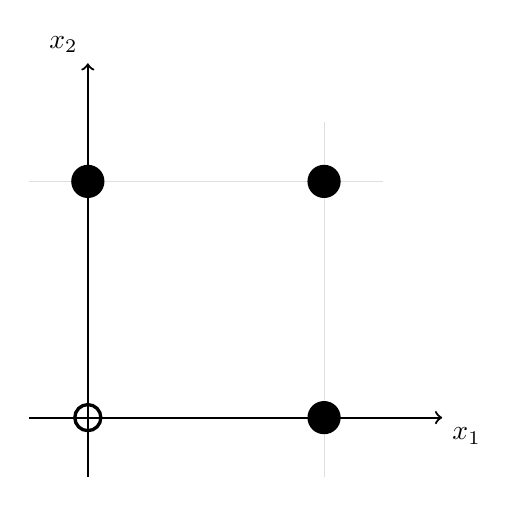
\begin{tikzpicture}[scale=3,auto]
        \draw[step=1cm,gray!25!,very thin] (-0.25,-0.25) grid (1.25,1.25);
        \draw[thick,->] (-0.25,0) -- (1.5,0) node[anchor=north west] {$x_1$};
        \draw[thick,->] (0,-0.25) -- (0,1.5) node[anchor=south east] {$x_2$};
        \node[circle,draw,very thick] (c) at (0,0){};
        \fill (1,0)  circle[radius=2pt];
        \fill (0,1)  circle[radius=2pt];
        \fill (1,1)  circle[radius=2pt];
    \end{tikzpicture}\quad
    \begin{tikzpicture}[scale=3,auto]
        \draw[step=1cm,gray!25!,very thin] (-0.25,-0.25) grid (1.25,1.25);
        \draw[thick,->] (-0.25,0) -- (1.5,0) node[anchor=north west] {$x_1$};
        \draw[thick,->] (0,-0.25) -- (0,1.5) node[anchor=south east] {$x_2$};
        \node[circle,draw,very thick] (c) at (0,0){};
        \fill (1,0)  circle[radius=2pt];
        \fill (0,1)  circle[radius=2pt];
        \node[circle,draw,very thick] (c) at (1,1){};
    \end{tikzpicture}
    \end{center}
    A single-layer perceptron can only learn linearly separable problems
\end{frame}


\begin{frame}{Adding a hidden layer}
    It is possible to do XOR, but we need to add a \textbf{hidden layer}
    \begin{center}
        \def\hhskip{4cm}
        \def\vvskip{4cm}
        \begin{tikzpicture}[scale=1, 
		every node/.style={transform shape},
		auto,
		cloud/.style={minimum width={width("N-1")+2pt},
			draw, ellipse},
		connected/.style={dotted,-}]
		%% Input nodes
		\node [cloud] at (0,0*\vvskip) (i1) {$0\lor 1$};
		\node [cloud] at (0,-1*\vvskip) (i2) {$0\lor 1$};
        %% Hidden node
        \node [cloud] at (1*\hhskip,-0.5*\vvskip) (h1) {$\theta=1$};
		%% Output node
		\node [cloud] at (2*\hhskip,-0.5*\vvskip) (o1) {$\theta=0$};
		%% Arcs
		\path [line] (i1) to node [midway, above, sloped] (TextNode) {$w=1$} (o1);
		\path [line] (i2) to node [midway, below, sloped] (TextNode) {$w=1$} (o1);
		\path [line] (i1) to node [midway, below, sloped] (TextNode) {$w=0.6$} (h1);
		\path [line] (i2) to node [midway, above, sloped] (TextNode) {$w=0.6$} (h1);
		\path [line] (h1) to node [pos=0.25, above] (TextNode) {$w=-2$} (o1);
	\end{tikzpicture}
    \end{center}
\end{frame}




\begin{frame}[fragile]\frametitle{Now the XOR truth table}
\begin{knitrout}
\definecolor{shadecolor}{rgb}{0.969, 0.969, 0.969}\color{fgcolor}\begin{kframe}
\begin{alltt}
\hldef{XOR_table} \hlkwb{=} \hlkwd{matrix}\hldef{(}\hlkwd{c}\hldef{(}\hlnum{0}\hldef{,} \hlnum{0}\hldef{,} \hlnum{0}\hldef{,}
                     \hlnum{1}\hldef{,} \hlnum{0}\hldef{,} \hlnum{1}\hldef{,}
                     \hlnum{0}\hldef{,} \hlnum{1}\hldef{,} \hlnum{1}\hldef{,}
                     \hlnum{1}\hldef{,} \hlnum{1}\hldef{,} \hlnum{0}\hldef{),}
                  \hlkwc{nc} \hldef{=} \hlnum{3}\hldef{,} \hlkwc{byrow} \hldef{=} \hlnum{TRUE}\hldef{)}
\hldef{XOR_table} \hlkwb{=} \hlkwd{as.data.frame}\hldef{(XOR_table)}
\hlkwd{colnames}\hldef{(XOR_table)} \hlkwb{=} \hlkwd{c}\hldef{(}\hlsng{"x1"}\hldef{,} \hlsng{"x2"}\hldef{,} \hlsng{"XOR"}\hldef{)}
\end{alltt}
\end{kframe}
\end{knitrout}
\end{frame}

\begin{frame}[fragile]\frametitle{Try to learn it without a hidden layer}
\begin{knitrout}
\definecolor{shadecolor}{rgb}{0.969, 0.969, 0.969}\color{fgcolor}\begin{kframe}
\begin{alltt}
\hldef{nn_XOR} \hlkwb{=} \hlkwd{neuralnet}\hldef{(XOR} \hlopt{~} \hldef{x1} \hlopt{+} \hldef{x2,}
                   \hlkwc{data} \hldef{= XOR_table,}
                   \hlkwc{act.fct} \hldef{=} \hlsng{"logistic"}\hldef{,}
                   \hlkwc{hidden} \hldef{=} \hlnum{0}\hldef{,}
                   \hlkwc{linear.output} \hldef{=} \hlnum{FALSE}\hldef{)}
\hldef{pred} \hlkwb{=} \hlkwd{predict}\hldef{(nn_XOR, XOR_table)}
\hldef{XOR_table}\hlopt{$}\hldef{result} \hlkwb{=} \hldef{pred} \hlopt{>} \hlnum{0.5}
\hlkwd{kable}\hldef{(XOR_table,} \hlsng{"latex"}\hldef{,} \hlkwc{booktabs} \hldef{=} \hlnum{TRUE}\hldef{)}
\end{alltt}
\end{kframe}
\begin{tabular}{rrrl}
\toprule
x1 & x2 & XOR & result\\
\midrule
0 & 0 & 0 & FALSE\\
1 & 0 & 1 & TRUE\\
0 & 1 & 1 & FALSE\\
1 & 1 & 0 & TRUE\\
\bottomrule
\end{tabular}

\end{knitrout}
\end{frame}

\begin{frame}[fragile]\frametitle{Now with a hidden layer}
\begin{knitrout}
\definecolor{shadecolor}{rgb}{0.969, 0.969, 0.969}\color{fgcolor}\begin{kframe}
\begin{alltt}
\hldef{nn_XOR} \hlkwb{=} \hlkwd{neuralnet}\hldef{(XOR} \hlopt{~} \hldef{x1} \hlopt{+} \hldef{x2,}
                   \hlkwc{data} \hldef{= XOR_table,}
                   \hlkwc{act.fct} \hldef{=} \hlsng{"tanh"}\hldef{,}
                   \hlkwc{hidden} \hldef{=} \hlnum{1}\hldef{)}
\hldef{pred} \hlkwb{=} \hlkwd{predict}\hldef{(nn_XOR, XOR_table)}
\hldef{XOR_table}\hlopt{$}\hldef{result} \hlkwb{=} \hldef{pred} \hlopt{>} \hlnum{0.5}
\hlkwd{kable}\hldef{(XOR_table,} \hlsng{"latex"}\hldef{,} \hlkwc{booktabs} \hldef{=} \hlnum{TRUE}\hldef{)}
\end{alltt}
\end{kframe}
\begin{tabular}{rrrl}
\toprule
x1 & x2 & XOR & result\\
\midrule
0 & 0 & 0 & FALSE\\
1 & 0 & 1 & TRUE\\
0 & 1 & 1 & TRUE\\
1 & 1 & 0 & TRUE\\
\bottomrule
\end{tabular}

\end{knitrout}
\vfill
Should look into options.. :)
\end{frame}

\begin{frame}[fragile]\frametitle{An example from the \code{neuralnet} manual -- Training vs testing sets}
\code{iris} is a built-in \code{R} dataset detailing physical characteristics of 150 flowers from 3 iris species
\vfill
\begin{knitrout}
\definecolor{shadecolor}{rgb}{0.969, 0.969, 0.969}\color{fgcolor}\begin{kframe}
\begin{alltt}
\hldef{train_idx} \hlkwb{<-} \hlkwd{sample}\hldef{(}\hlkwd{nrow}\hldef{(iris),} \hlnum{2}\hlopt{/}\hlnum{3} \hlopt{*} \hlkwd{nrow}\hldef{(iris))}
\hldef{iris_train} \hlkwb{<-} \hldef{iris[train_idx, ]}
\hldef{iris_test} \hlkwb{<-} \hldef{iris[}\hlopt{-}\hldef{train_idx, ]}
\end{alltt}
\end{kframe}
\end{knitrout}
\vfill
Thus we pick at random 2/3 of the data for training and 1/3 for testing. See some considerations on training, validation and testing on \href{https://en.wikipedia.org/wiki/Training,_validation,_and_test_data_sets}{this Wikipedia page}
\end{frame}

\begin{frame}[fragile]\frametitle{An example from the \code{neuralnet} manual}
\begin{knitrout}
\definecolor{shadecolor}{rgb}{0.969, 0.969, 0.969}\color{fgcolor}\begin{kframe}
\begin{alltt}
\hldef{nn} \hlkwb{<-} \hlkwd{neuralnet}\hldef{(Species} \hlopt{==} \hlsng{"setosa"} \hlopt{~} \hldef{Petal.Length} \hlopt{+} \hldef{Petal.Width,}
                \hldef{iris_train,} \hlkwc{linear.output} \hldef{=} \hlnum{FALSE}\hldef{)}
\hldef{pred} \hlkwb{<-} \hlkwd{predict}\hldef{(nn, iris_test)}
\hlkwd{table}\hldef{(iris_test}\hlopt{$}\hldef{Species} \hlopt{==} \hlsng{"setosa"}\hldef{, pred[,} \hlnum{1}\hldef{]} \hlopt{>} \hlnum{0.5}\hldef{)}
\end{alltt}
\begin{verbatim}
##        
##         FALSE TRUE
##   FALSE    37    0
##   TRUE      0   13
\end{verbatim}
\end{kframe}
\end{knitrout}
\end{frame}

\begin{frame}[fragile]\frametitle{Another example -- multiclass classification}
\begin{knitrout}
\definecolor{shadecolor}{rgb}{0.969, 0.969, 0.969}\color{fgcolor}\begin{kframe}
\begin{alltt}
\hldef{nn} \hlkwb{<-} \hlkwd{neuralnet}\hldef{((Species} \hlopt{==} \hlsng{"setosa"}\hldef{)} \hlopt{+}
                  \hldef{(Species} \hlopt{==} \hlsng{"versicolor"}\hldef{)} \hlopt{+}
                  \hldef{(Species} \hlopt{==} \hlsng{"virginica"}\hldef{)}
                 \hlopt{~} \hldef{Petal.Length} \hlopt{+} \hldef{Petal.Width,}
                \hldef{iris_train,} \hlkwc{linear.output} \hldef{=} \hlnum{FALSE}\hldef{)}
\hldef{pred} \hlkwb{<-} \hlkwd{predict}\hldef{(nn, iris_test)}
\hlkwd{table}\hldef{(iris_test}\hlopt{$}\hldef{Species,} \hlkwd{apply}\hldef{(pred,} \hlnum{1}\hldef{, which.max))}
\end{alltt}
\begin{verbatim}
##             
##               1
##   setosa     13
##   versicolor 19
##   virginica  18
\end{verbatim}
\end{kframe}
\end{knitrout}
\end{frame}

\end{document}
